% !Mode\dots ``TeX:UTF-8''
\documentclass[10pt,a4paper]{article}

\usepackage{comment}
\usepackage{amsmath}
\usepackage{amssymb}
\usepackage{amsthm}
\usepackage{amscd}
\usepackage{graphicx}
\usepackage{indentfirst}
\usepackage{breqn}
\usepackage[ruled, vlined, linesnumbered]{algorithm2e}
\usepackage{titlesec}
\usepackage[top=25.4mm,  bottom=25.4mm,  left=31.7mm,  right=31.2mm]{geometry}
%\usepackage{geometry}
\usepackage{titlesec}
\usepackage{color}
\parskip 1.0mm
   \usepackage{amsmath, amssymb}
   \usepackage{latexsym}
   \newcommand{\mycite}[1]{$^{\mbox{\rm\scriptsize\cite{#1}}}\!$}

\usepackage{float}
\usepackage{url}
%\usepackage{yfonts}
\usepackage{comment}
\usepackage{amsfonts}
\usepackage{latexsym,amsmath,epsfig,amssymb,graphics}
\usepackage{caption}

\usepackage[T1]{fontenc}
\usepackage[utf8]{inputenc}
\usepackage{authblk}



%\usepackage[ruled]{algorithm2e}
\renewcommand{\algorithmcfname}{ALGORITHM}
\SetAlFnt{\small}
\SetAlCapFnt{\small}
\SetAlCapNameFnt{\small}
\SetAlCapHSkip{0pt}
\IncMargin{-\parindent}



%The following is my definie symbol
\def \froot {{\tt logcf}}
\def \MM {{\tt Mathematica}}
\def \MAPLE {{\tt Maple}}
\def \inte {{\tt RootIntervals}}
\def \cf {{\tt CF}}
\def \sle {{\tt Sleeve}}
\def \eign {{\tt eigensolve}}
\def \AND {{\tt ANewDsc}}
\def \SLV {{\tt SLV}}

%\def \MPS{ {\tt MPSolve}}
\def \REALROOT {{\tt realroot}}

\def \ZZ {{\mathbb Z}}

\def \RR {{\mathbb R}}

\def \algcf{{\tt cf}}
\def \sign{{\rm sign}}
\def \abs {{\rm abs}}
\def \gcd {{\rm gcd}}
\def \deg {{\rm deg}}
\def \algm{{\tt main}}
\def \dec {{\tt dec}}
\def \up {{\tt logup}}

\def \less {{\tt lessOne}}
\def \lb {{\tt loglb}}



%\newdef{rmk}{Remark}
%\newproof{pf}{Proof}
%\newproof{pot}{Proof of Theorem \ref{thm2}}


\newtheorem{note}{Notation}
\newtheorem{theorem}{\bf Theorem}
\newtheorem{definition}{\bf Definition}
\newtheorem{corollary}{\bf Corollary}
\newtheorem{example}{\bf Example}
\newcommand{\rev}[1]{{\color{red}{#1}}}
\graphicspath{{img/}}



% Document starts
\begin{document}


	
	% Title portion
	\title{\froot: An Efficient Tool for Real Root Isolation}
		
		\author[1]{Liyun Dai\thanks{dailiyun@swu.edu.cn. Corresponding author}	}
		\author[2]{Bican Xia \thanks{xbc@math.pku.edu.cn}}
		\affil[1]{RISE, Southwest University, Chongqing, China}
		\affil[2]{LMAM \& School of Mathematical Science\  Peking University,  Beijing,  China}
	
	\renewcommand\Authands{ and }
\date{}
\maketitle

\begin{abstract}
  %This paper revisits an   algorithm for isolating real roots of  univariate
  %polynomials based on continued fractions. It follows  the work of Vincent,	Uspensky, Collins and Akritas, Johnson and Krandick.
Computing upper bounds of the positive real roots of some polynomials is a key step of those real root isolation algorithms based on continued fraction expansion and Vincent's theorem. We give a new algorithm  for computing an upper bound of positive roots in this paper. The complexity of the algorithm is  $O(n\log(u+1))$ \rev{addition and multiplication symbolic operators}  where $u$ is the optimal upper bound satisfying Theorem \ref{thm:log} of this paper and $n$ is the degree of the polynomial. Our method together with some tricks has been implemented as a  software package \froot\ using \texttt{C} language. Experiments on many benchmarks show that \froot \  is competitive with \inte\ of \MM\ and  the function \REALROOT\ of \MAPLE\ averagely and it also much faster than  state of art open source real root solvers in many test cases.
~\\
{\bf Keywords: }
univariate polynomial,  real root isolation, continued fractions,  computer algebra
\end{abstract}


\section{Introduction }
\label{}
Real root isolation of univariate polynomials with integer coefficients is one of the fundamental tasks in computer algebra as well as in many applications ranging from computational geometry to quantifier elimination. The problem can be stated as: given a polynomial $p\in \ZZ[x]$, compute for each of its real roots an interval with rational endpoints containing it and being disjoint from the intervals
computed for the other roots.  There are three methods to isolate real root.  The first kind consists of the subdivision algorithms using counting techniques based  on, {\it e.g.}, the Strum theorem or
Descartes' rule of signs.  This  method counts the sign changes (of Sturm sequence or coefficients of some polynomials) in the considered interval and if the sign changes reach $1$ or $0$, the procedure returns from this interval.
Otherwise it subdivides the interval and compute recursively. The symbolic implementations of this method can be found in \cite{collin76,rou04,kobel2016computing,Tsigaridas2016} and the symbolic-numberic algorithms implementations can be found in \cite{rou04,eig05,eig08,meh11}.

The second kind method takes use of the continued fraction algorithms \cite{akr08,tsi08,sha08}. These methods are highly efficient and competitive \cite{rou04,hemmer09}. Especially,  \cite{hemmer09} provides a test dataset   consisting of 5000 polynomials from many
different settings,  with results indicating that there is no best method overall.
%However one can say that for most instances the solvers based on  continued fraction are among
%the best methods.
%{\color{blue}{In this paper, based on a new upper bound on positive roots of univariate polynomials and some tricks, we give a continued fraction based algorithm for real root isolation and a more efficient tool, called \froot.}}

The third method is based on Newton-Raphson method and interval arithmetic.
The search space is subdivided until it contains only a single real root and Newton's method converges. When the polynomial is sparse and has very high degree, this method will be much faster than other methods. The symbolic implementations of this kind of methods can be found in \cite{xia06,xia07} and the numeric implementations
can be found in \cite{kla93,rump99}.

Those methods, which are  based on  continued fraction compute the continued fraction expansion of the real roots of a polynomial so as to  compute isolating intervals for real roots. One important step
is to  compute the upper bounds of the positive real roots of some polynomials. There are  several classic methods to compute such upper bounds, such as Cauchy bounds, Lagrange-MacLaurin  bounds and Kioustelidis' bounds. And there are many recent works about the upper bound of the positive roots of univariate polynomials \cite{hong98,ste05,akr08}. Some methods for computing these bounds,  such as Cauchy bounds, are of $O(n)$ complexity but the results are very coarse. Some methods, as presented in  \cite{akr08} are of $O(n^2)$ complexity but their bounds are sharper. The balance between the precision and effect for computing such upper bounds has to be taken into account.

We provide a new method for computing such bounds with time complexity $O(n\log(u+1))$, where $u$ is the optimal upper bound satisfying Theorem \ref{thm:log}. Besides, compared
with \cite{akr08}, when  Algorithm \ref{alg:less} return true (the upper bound is less than $1$), our upper bound is at most two times that in \cite{akr08}. In this way, the algorithm of   isolating real roots is improved.  Our  method has been implemented as a  software package \froot\ using \texttt{C} language. For many benchmarks \froot \  is about four  times
faster   than  the function {\tt \REALROOT} of \MAPLE. Roughly speaking, \froot\ is competitive with \inte\ of \MM. In some test cases \froot\ is faster than \inte\ but in some other cases \inte\ is faster than \froot\ and the mean time of all test cases is almost the same. But we have an interesting finding that {\tt \inte} may output wrong results on some input polynomials due to incorrect zero judgement. %And it  is also much faster than   open source real root solver.}
And in general \froot\ is also much faster than other state of art
open source exact real root isolation solvers, such as \cf, \AND and \SLV. For those  benchmarks which  have only real roots, \froot\ is much faster than \sle\ and \eign\ which are based on numerical computation.


The rest of this paper is organized as follows. Section 2 reviews the
main algorithm for real root isolation based on  continued fraction. Section 3 presents a new algorithm for
computing an upper bound of positive roots. Section 4 lists some tricks used in \froot.  Section 5 lists the comparative experimental results of our algorithm and other software. %The paper is concluded in Section 5.


% !Mode\dots ``TeX:UTF-8''

\section{Algorithm based on  continued fraction}
\label{sec:contalg}
In this section, we first recall {\em Descartes' rule of signs}, which gives a bound on the number of positive real roots. Then the {\em Vincent theorem}, which  ensures
the termination of algorithms based on  continued fractions, is presented. Finally, we review an algorithm of real root isolation based on  continued fractions.


As usual, $\deg(p)$ denotes the degree of univariate polynomial $p$. The derivative of polynomial $p$ with respect to the only variable is denoted by $p'$ and $\gcd(f,g)$ means the greatest common divisor of polynomials $f$ and $g$.
\rev{
\begin{example}
	\label{ex:exp1}
	Consider the polynomial
	\[p_1(x)=x^6+2x^5-4x^4+x^3+10x^2-5x+5.\]
	\[\deg(p_1)=6, p_1'=6x^5+10x^4-16x^3+3x^2+20x-5.\]
\end{example}
}

\begin{note}[Sign variation]
Let $S=\left\{ a_0,a_1,\ldots,a_n \right\}$ be a finite sequence of non-zero real numbers. Define $V(S)$, the {\em sign variation} of $S$, as follows.
\[V(S)=0\ \text{ if } |S|\le1,\]
\[  V(a_0,\ldots,a_{n-1},a_n)=  \left\{\begin{aligned}
 &  V(a_0,\ldots,a_{n-1})+1 \text{ if }a_{n-1}a_n<0;\\
&V(a_0,\ldots,a_{n-1}), \text{ otherwise}.\\
	\end{aligned}
	\right.
\]
If some elements of $S$ are zero, remove those zero-elements to get a new sequence and define $V(S)$ to be the sign variation of this new sequence.

\end{note}



%\rev{There are many studies about  real roots for a given polynomial,  and {\em Descartes' rule of signs} is one of beautiful results among them.  It  provides an upper bound of the number of positive real roots.}


\begin{theorem}[Descartes' rule of signs] \label{thm:des}
  Suppose $p=\sum_{i=0}^na_ix^i\in\RR[x]$ has $m$ positive real roots, counted with multiplicity. Set $V(p)=V(a_0,a_1,\ldots,a_n)$. Then $m\le V(p)$, and $V(p)-m$ is even.
\end{theorem}

%\rev{ For {\em Example \ref{ex:exp1}}, $V(p_1)=V(5,-5,10,1,-4,2,1)=4$.  {\em Descartes' rule of signs} is an useful tool to estimate the number of  real roots. And if $V(p)=1$, then employ this rule, there is exact one  positive root.  But when $V(p)>1$, the rule can not directly isolate the real roots. {\em Vincent's theorem} in the following will overcome this restriction. {\em Vincent's theorem} says that if we give a small enough interval, then it can map this interval to entire positive domain and $V(p)\le 1$.}



\begin{theorem}[Vincent's theorem]\label{thm:vin}
  Let $p(x)$ be a real polynomial of degree $n$ which has only simple roots. It is possible to determine a positive quantity $\delta$ so that for every pair of positive real numbers $a$ and $b$ with $|b-a| < \delta$, the coefficients sequence of every transformed polynomial of the form
  $  p(x) = (1+x)^{n}p(\frac{a+bx}{1+x}) $
		  has exactly 0 or 1 sign variation. The second case is possible if and only if $p(x)$ has a single root within $(a,b)$.
\end{theorem}

\begin{definition}  We define the following transformations for a univariate polynomial $p(x)=a_nx^n+a_{n-1}x^{n-1}+\cdots+a_1x+a_0,n>0$.
  \begin{eqnarray*}
  lc(p(x))&=&a_n,\\
  R(p(x))&=&x^n(p(\frac{1}{x})),\\
  H_\lambda(p(x))&=&p(\lambda x),\\
  T(p(x))&=&p(x+1), \\
  D(p(x))&=&a_nx^{n-1}+a_{n-1}x^{n-2}+\cdots+a_2x+a_1.
  \end{eqnarray*}
\end{definition}

$T(p)$  is also called	{\em Taylor shift one} \cite{ger04,joh05}.

\begin{algorithm}
\SetAlgoCaptionSeparator{.}
\caption{\algm \label{alg:main}}
\DontPrintSemicolon
\KwIn{ A non-zero polynomial $p(x)\in \ZZ[x] $. }
\KwOut{$I$,  a set of real root isolating intervals of $p(x)$. }
$I=\emptyset$; \;
\If {$\deg(p)$  equals to $0$}  {return $I$;}
$p=\frac{p}{\gcd(p,p')}$; \tcc{ square free}
\If {$p(0)$   equals to  $0$ } { $I.add([0,0])$; \tcc{ add $[0,0]$ to set $I$}
$p=D(p)$; \tcc{derivative of $p$ }
}
$I$.addAll(\algcf($p$)); \;
\tcc { add all the positive root intervals to set $I$ } \tcc{ \algcf\ is described as {\em Algorithm \ref{alg:cf}}}
$p=p(-x)$;\;
$I$.addAll(-\algcf($p$));
\end{algorithm}


%In our experiments when {\em Algorithm \ref{alg:up}} is used for computing upper bounds, $T(p)$  takes  more than ninety percent of running time\footnote{The result of  GNU gprof.}.  We have considered methods in \cite{ger04} for computing $T(p)$, but   finally we chose the  classical method (Horner's method) for its simplicity. In future work we will use Divide \& Conquer method which is the fastest in \cite{ger04}. We think \rev{further} substituting will still improve the performance of our method.
{\em Vincent's theorem} provides  a possible method to isolate the real roots. But it needs to divide $\RR$ into  many small intervals and the width of these intervals is smaller than a given  finite value. So {\em Vincent's theorem} cannot be used to isolate the real roots directly since $\RR$ is infinite. For employing  {\em Vincent's theorem}, we need to discard the intervals containing no real roots. {\em Algorithm \ref{alg:lb}} provides a lower  bound $lb$ of positive roots for given $p$.  Since the interval  $(0,lb)$ contains no real roots,  we can safely  discard $(0,lb)$ when isolate the real roots.


\begin{algorithm}
\SetAlgoCaptionSeparator{.}
\caption{\lb \label{alg:lb}}
\DontPrintSemicolon
\KwIn{ $p\in\ZZ[x],\ lc(p)\neq 0 $. }
\KwOut{$root\_lb$, a lower bound of positive roots of $p$. }
$p=R(p)$;\;
\lIf{$lc(p)<0$}{	$p=-p$;}
$root\_lb=$\up($p$); \tcc{\up\ is described as {\em Algorithm \ref{alg:up}}}
\end{algorithm}


\begin{definition}
$  intvl(a,b,c,d)=  \left\{\begin{aligned}
&  (\min\left\{ \frac{a}{c},\frac{b}{d} \right\},\ \max\left\{ \frac{a}{c},\frac{b}{d} \right\} ) &\text{ if } cd\neq0;\\
& (0,\infty), &\text{ otherwise}.\\
	\end{aligned}
	\right.
$
\end{definition}


Using the above notations and definitions, an algorithm for isolating all the real roots of a nonzero univariate polynomial is described as {\em Algorithm \ref{alg:main}}.
{\em Algorithm \ref{alg:cf}}, which is a slight modification of the algorithm in \cite{akr08}, is presented here to make our subsequent description clearer.

Continued fractions based procedures will continue subdividing the considered interval into two subintervals and make a one to one map from $(a,b)$ to $(0,+\infty)$ by $  p(x) = (1+x)^{n}p(\frac{a+bx}{1+x})$ until $V(p)$ equals $1$ or $0$. Informally, {\em Algorithm \ref{alg:main}} is employing the above map to magnify the considered interval  to $(0,+\infty)$.  Through {\em Descartes' rule of signs}, there is no positive real roots if  $V(p)=0$. In this case we delete the interval from the considered interval set.   When $V(p)=1$, this interval contains exact one real root by {\em Descartes' rule of signs}. In this case we throw away the interval from the considered interval set. When $V(p)>1$, since it cannot be determined how many real roots are contained in this interval, we divide the considered interval into two subintervals. In this case we throw away the interval from the considered interval set and add two subintervals to the considered interval set. Repeating this procedure, we can divide the interval into  subintervals until  there is no width of  the corresponding original interval greater or equal to $\delta$ in considered interval set.   Then there is at most one real root in every interval in the considered interval set and then the procedure will terminate. This is also
the reason why {\em Theorem \ref{thm:vin}}  can guarantee the termination of {\em Algorithm \ref{alg:main}}.



\begin{algorithm}
	\SetAlgoCaptionSeparator{.}
	\caption{\algcf \label{alg:cf}}
	\DontPrintSemicolon
	\KwIn{ A squarefree polynomial $p \in \ZZ[x] \setminus \{0\}$. }
	\KwOut{ $roots$, a list of isolating intervals of positive roots of $p$. }
	
	$roots=\emptyset$;
	$s=V(p)$;\;

	$intstack=\emptyset$;
	$intstack$.add($\{1,0,0,1,p,s\}$);\;
	\While{$intstack\neq \emptyset$} {
		$\{a,b,c,d,p,s\}=intstack.$pop();\tcc{pop  the first element}
		$\lambda=\lb(p)$;\;
		\lIf{$\lambda \ge 1$ \label{log:branch}}{
			$\{ a,c,p \}=\{ \lambda  a,\lambda c ,H_\lambda(p) \}$;
			$\{ b,d,p \}=\{   a+b,c+d ,T(p) \}$;\;
			\lIf { $p(0)= = 0$}{
				$roots$.add$([\frac{b}{d},\frac{b}{d}])$ ;
				$p=\frac{p}{x}$;}
			$s=V(p)$;
			\lIf {$s= = 0$}{
				continue;
			}
			\lElseIf{$s= = 1$}{		
				$roots$.add($intvl(a,b,c,d)$);
				continue;
			}
		}
		$ \left\{ p_1,a_1,b_1,c_1,d_1,r \right\}=\left\{ T(p),a,a+b,c,c+d,0 \right\}$
		
		\lIf{$p_1(0)= =0$}{
			$roots$.add($[\frac{b_1}{d_1},\frac{b_1}{d_1}]$);
			$p_1=\frac{p_1}{x};r=1$;
		}
		$s_1=V(p_1)$;
		$\left\{ s_2,a_2,b_2,c_2,d_2 \right\}=\left\{ s-s_1-r,b,a+b,d,c+d \right\}$;
		%$ s_2 = s- s_1 - r; a_2 = b; b_2 = a + b; c_2 = d; d_2 = c + d$;\;
		\lIf {$s_2>1$ }{
			$ p_2= (x+1)^{\deg(p)}T(p)$;\;
			\lIf {$p_2(0)= = 0$}{
				$p_2=\frac{p_2}{x}$;
				$s_2=V(p_2)$;
			}
		}
		\lIf{$s_1= = 1$ }{
			$roots$.add($intvl(a_1,b_1,c_1,d_1)$);\;
		}
		\lElseIf{$s_1>1$ }{
			$intstack$.add($\{a_1,b_1,c_1,d_1,p_1,s_1\}$);\;
		}
		
		\lIf{$s_2= = 1$}{
			$roots$.add($intvl(a_2,b_2,c_2,d_2)$);\;
		}
		\lElseIf{$s_2>1$ }{
			$intstack$.add($\{a_2,b_2,c_2,d_2,p_2,s_2\}$);\;
		}
	}
\end{algorithm}




%\newpage
\section{A new upper bounds of the positive real roots for giving  polynomials}
\label{sec:thm}

One key ingredient of continued fraction based methods is the computation of upper bounds of the positive real roots for giving  polynomials. We give in {\em Theorem \ref{thm:log}} a new characteristic of such upper bounds of univariate polynomials. A new algorithm based on this theorem, {\em Algorithm \ref{alg:up}}, is proposed for computing upper bounds of positive real roots.


\begin{theorem} 
	\label{thm:log}
  Suppose   $p=a_nx^n+a_{n-1}x^{n-1}+\cdots+a_1x+a_0\ (a_n>0)$  is a univariate polynomial in $x$ with real coefficients.  Then  a nonnegative number $u$ is an upper bound of positive roots of $p$ if $u$   satisfies that $\min_{j=0}^{n}\left\{  \sum_{i=j}^n a_i u^{i-j}\right\}\ge0$.
\end{theorem}
\begin{proof}
  If $n=0$, then $p$ is a nonzero constant and any positive number is its upper bound of positive roots.

  Otherwise, if $b>u$,  we {\bf claim} that $\sum_{i=j}^na_ib^{i-j}> \sum_{i=j}^na_iu^{i-j}$ for any $j= 0,\ldots,n-1$.

  When $j=n-1$, $\sum_{i=n-1}^na_ib^{i-n+1}-\sum_{i=n-1}^na_iu^{i-n+1}=a_n(b-u)>0.$ The claim holds.

  Assume the {\bf claim} holds  when $j=k$. When $j=k-1$,  $\sum_{i=k-1}^na_ib^{i-k+1}=\left(\sum_{i=k}^na_ib^{i-k}\right)b+a_{k-1} $. By assumption
  $\sum_{i=k}^na_ib^{i-k}>\sum_{i=k}^na_iu^{i-k}\ge0$. Since $b>u\ge0$, $\left(\sum_{i=k}^na_ib^{i-k}\right)b>\left (\sum_{i=k}^na_iu^{i-k} \right)u  $
  and $\sum_{i=k-1}^na_ib^{i-k+1}> \sum_{i=k-1}^na_iu^{i-k+1}$. So  $\sum_{i=j}^na_ib^{i-j}> \sum_{i=j}^na_iu^{i-j}$ for any $j= 0,\ldots,n-1$.


  By the above claim,   $p(b)=\sum_{i=0}^na_ib^i>0$ when  $b>u$. Because $b$ is arbitrarily chosen, $u$ is an upper bound of the positive roots of $p$.

\end{proof}

\rev{For {\em Example \ref{ex:exp1}},  two real roots of equation $x^2-x-4$ are $-1-\sqrt{5}$ and $-1+\sqrt{5}$. And the largest real root of $x^5+2x^4-x^3+x^2+10x-5$ is less than $1$. Hence, $\min\{x\mid  \sum_{i=j}^6 a_i u^{i-j} \ge 0, j=0\cdots,6 \} =-1+\sqrt{5}$.  } 


The following theorem was given by Akritas et al. in  \cite{akr08}, which computes positive root upper bounds of univariate polynomials.

\begin{theorem}[Akritas-Strzebo\'{n}ski-Vigklas, \cite{akr08}]
	 \label{thm:qup}

  Let $p(x)=a_nx^n+a_{n-1}x^{n-1}+\cdots+a_0\ (a_n>0)$ be a polynomial with real coefficients and let $d(p)$ and $t(p)$ denote the degree and the number of its terms, respectively.

  Moreover, assume that $p(x)$ can be written as\begin{equation}
	p(x)=q_1(x)-q_2(x)+q_3(x)-q_4(x)+\cdots +q_{2m-1}(x)-q_{2m}(x)+g(x)
	\label{eq:1}
  \end{equation}
  where all the coefficients of polynomials $q_i(x)$ $(i=1,2,\ldots,2m)$ and $g(x)$ are positive. In addition,
  assume that for $i=1,2,\ldots,m$ we have
  \begin{equation*}
	q_{2i-1}(x)=c_{2i-1,1}x^{e_{2i-1,1}}+\cdots+c_{2i-1,t_{2i-1}}x^{e_{2i-1,t_{2i-1}}}
  \end{equation*}
  and
  \begin{equation*}
	q_{2i}(x)=b_{2i,1}x^{e_{2i,1}}+\cdots+b_{2i,t_{2i}}x^{e_{2i,t_{2i}}}
  \end{equation*}
  where $e_{2i-1,1}=d(q_{2i-1})$, $e_{2i,1}=d(q_{2i})$, $t_{2i-1}=t(q_{2i-1}),$ and $t_{2i}=t(q_{2i})$   and the exponent of each term in $q_{2i-1}(x)$ is greater than the exponent of each term in $q_{2i}(x)$. If for all indices $i=1,2,\ldots,m$, we have
  \begin{equation*}
	t(q_{2i-1})\ge t(q_{2i}),
  \end{equation*}
  then an upper bound of the values of the positive roots of $p(x)$ is given by

  \begin{equation}\label{eq:2}
	up= \max_{i=1,2,\ldots,m}\left\{ \max_{j=1,2,\ldots,t_{2i}}\left\{ \left( \frac{b_{2i,j}}{c_{2i-1,j}} \right)^{\frac{1}{e_{2i-1,j}- e_{2i,j} } } \right\}  \right\}
  \end{equation}
  for any permutation of the positive coefficients $c_{2i-1,j}, $ $j=1,2,\ldots,t_{2i-1}$.
  Otherwise, for each of the indices $i$ for which we have
  \begin{equation*}
	t_{2i-1}<t_{2i},
  \end{equation*}
  we {\bf break up} one of the coefficients of $q_{2i-1}(x)$ into $t_{2i}-t_{2i-1} +1$ parts, so that now $t(q_{2i} ) = t(q_{2i-1})$ and apply the same formula (\ref{eq:2}) given above.


\end{theorem}
\rev{

For {\em Example \ref{ex:exp1}} we have
  \begin{eqnarray*}
 q_1&=&x^6+2x^5\\  	
 -q_2&=& -4x^4\\
 q_3&=& x^3+10x^2\\
 -q_4&=& -5x\\
 q_5&=&5.
  	\end{eqnarray*}
  	A direct application of {\em Theorem \ref{thm:qup}} pairs the terms $\{x^6, -4x^4\}$ of $q_1(x)$ and $q_2(x)$, and ignores the last term
  	of $q_1(x)$. For $q_3(x)$ and $q_4(x)$,   application of {\em Theorem \ref{thm:qup}} pairs the terms $\{x^3, -5x\}$ of them, and igonores the last  term of $q_3(x)$. The resulting upper bound is $\sqrt{5}$. As $\sqrt{5}< -1+\sqrt{5}$, in {\em Example \ref{ex:exp1}}, the upper bound given by {\em Theorem \ref{thm:qup}} is less than  the upper bound given by {\em Theorem \ref{thm:log}}. For the upper bound, the value is better if the estimated upper better is smaller. So in this case,  {\em Theorem \ref{thm:log}} is better than   {\em Theorem \ref{thm:qup}} }. In general, we shall show in {\em Theorem \ref{thm:com}} that the optimal bound given by {\em Theorem \ref{thm:log}} is better than that given by {\em Theorem \ref{thm:qup}}.









\begin{theorem}\label{thm:com}
	Let $p(x)=a_nx^n+a_{n-1}x^{n-1}+\cdots+a_0\ (a_n>0)$ be a polynomial with real coefficients and   $u$ denote an upper bound of positive roots of $p$ obtained by {\em Theorem \ref{thm:qup}}, then $\min_{k=0}^{n}\left\{  \sum_{i=k}^n a_i u^{i-k}\right\}\ge0$.
	
\end{theorem}

\begin{proof}

	For every $ a_i<0$, by {\em Theorem \ref{thm:qup}}, there exist  $c_{i_1}x^{e_{i_1}}$ and $b_{i_2}x^{e_{i_2}},$  respectively, such that
	$e_{i_1}>e_{i_2}$, $b_{i_2}x^{e_{i_2} }$ is the term $-a_ix^i$
	and $c_{i_1}x^{e_{i_1} }$ is either a whole or a part (broken up by {\em Theorem \ref{thm:qup}}) of a positive term of $p$. Since $u$ satisfies equation (\ref{eq:2}),
	 $c_{i_1}u^{e_{i_1}}\ge b_{i_2}u^{e_{i_2}}$.  
\rev{	 So $p(x)$ can be written as $p(x)=\sum (c_{i_1}x^{e_{i_1}}-b_{i_2}x^{e_{i_2}})$ where $c_{i_1}> 0,e_{i_1}> e_{i_2}, e_{{i+1}_1}\ge e_{i_1} $.
	 So for  every  $a_j>0$, the sum of coefficient $c_{i_1}$ where  the terms of $c_{i_1}x^{e_{i_1}}$    has a corresponding $ b_{i_2}x^{e_{i_2}}$ and $e_{i_1}=j$ is less or equal than $a_j$. In other words,

	for every  $a_j>0$,   $\left( \sum_{a_i<0,e_{i_1}=j }c_{i_1} \right)\le a_{j}$. So 
	\[\sum_{i=k}^na_iu^i\ge \sum_{i=k,a_i<0, a_ix^i=-b_{i_2}x^{e_{i_2}}  }^n \left( c_{i_1}u^{e_{i_1}}-
		b_{i_2}u^{e_{i_2}} \right)\ge 0 \] }for any $k= 0,1,\ldots,n$. Since $u\ge0$,  $\sum_{i=k}^n a_i u^{i-k}\ge0 $ for any  $k= 0,1,\ldots,n$ and \\ 
	$\min_{k=0}^{n}\left\{  \sum_{i=k}^n a_i u^{i-k}\right\}\ge0$.
\end{proof}



%\begin{theorem}\label{thm:com1}
%	
%	Let $p(x)=a_nx^n+a_{n-1}x^{n-1}+\cdots+a_0\ (a_n>0)$ be a polynomial with real coefficients. Let  $u_1$ denote the optimal upper bound of
%	positive real roots satisfying {\em Theorem \ref{thm:log}} and $u_2$ denote the optimal upper bound of positive real roots satisfying {\em Theorem \ref{thm:qup}}, then $u_1\le u_2$ and the  strict inequality can hold.
%\end{theorem}
%
%\begin{proof}
%	By {\em Theorem \ref{thm:com}}, $u_1\le u_2$.
%	Let $p(x)=x^2+x-2$. Then $u_2=\sqrt{2}$ and $u_1=1$. So
%	$u_1<u_2$ for this \rev{$p$}.
%\end{proof}




\section{Experiments}
%\subsection{Implementation}

%\subsection{Environment}

We first explain the implementation and computation environment.

{\bf Old environment}\ \ \
The main algorithm for isolating real roots based on our improvements has been implemented as a \texttt{C} program, \froot \footnote{The program can be downloaded through \url{https://github.com/djuanbei/logcf}}. Compilation was done using {\tt gcc} version 4.6.3 with optimization flags -O2.
We use {\tt Singular} \cite{singular} to read polynomials from files or standard input and to eliminate multi-factors of polynomials. We use the GMP\footnote{ \url{http://gmplib.org/}}
(version 5.05), arbitrary-length integers libraries, to deal with big integer computation.
Some tests were done before 2014   on a 64-bit Intel(R) Core(TM) i5 CPU 650 @ 3.20GHz with 4GB RAM memory and Ubuntu 12.04 GNU/Linux.

{\bf New environment}\ \ \
Since   source code and execution files
	of    \eign, \cf\ and \sle\  cannot be found in public area so far, we only compare \froot\ with \AND, \MM's \inte\  and  \MAPLE's \REALROOT\  on   a 64-bit Intel(R) Core(TM) i7 CPU-4710Q @ 2.50GHz with 8GB RAM memory and Windows 7. In this environment \froot\ was compiled by visual studio 2013.

\subsection{Benchmarks }
 \subsubsection{$W_n$}
 {\it Wilkinson} polynomials: $W_n=\Pi_{i=1}^n(x-i)$. %The integers $1,2,\ldots,n $ are  all the real roots of $W_n$.
  \subsubsection{$mW_n$}
  %{\it Wilkinson}  polynomials have a fine property  of containing only rational roots, which most of the polynomials do not have . So we modify
  Modified {\it Wilkinson} polynomials: $mW_n=W_n-1$.

  If $n>10$, $mW_n$ has $n$ simple real roots but most of them are irrational.
 \subsubsection{$IW_n$}
 The distance between  $W_n$'s two  nearest real roots  is  $1$ and the distance between $mW_n$'s two nearest real roots  is nearly $1$. %Their real roots distribution   tends to be  uniform.  So
 We construct new polynomials $IW_n=\Pi_{i=1}^n(ix-1)$, which have a completely different nearest distance. % between any two nearest real roots.
 \subsubsection{$ mIW_n$ }
 We modify $IW_n$  into $mIW_n=IW_n-1$ for the same purpose  as we construct $mW_n$. Most real roots of $mIM_n$  become irrational.
 \subsubsection{$T_n$} {\it ChebyshevT} polynomials: $T_0=1,T_1=x,T_{n+1}=2xT_n-T_{n-1}$. $T_n$ has $n$ simple real roots.
 \subsubsection{$U_n$} {\it ChebyshevU} polynomials: $U_0=1,U_1=2x,U_{n+1}=2xU_n-U_{n-1}$. $U_n$ has $n$ simple real roots.
 \subsubsection{$L_n$}
 {\it Laguerre}  polynomials: $L_0=1$,$L_1=1-x$,$L_{n+1}(x)=\frac{  (2n+1-x )L_n(x)-  nL_{n-1 }(x)}{(n+1) }$. %We can
 %modify  it to  integer polynomial through multiplying   by  $n!L_n$.
Obviously, $n!L_n$ is a polynomial with integer coefficients.
 \subsubsection{$M_n$} {\it Mignotte} polynomials: $x^n-2(5x-1)^2$. If $n$ is odd, $M_n$ has three simple real roots. If $n$ is even, it has four simple real roots.

\subsubsection{$MR_n$}{\it Mignotte} rational center polynomials: $ x^n-((2^7-1)x-1)^2$.
	
 \subsubsection{$H_n$}{\it Hermite } polynomials:  $H_0=1,H_1=2x,H_n=2xH_{n-1}-2(n-1)H_{n-2}$. $H_n$ has $n$ simple real roots.

 \subsubsection{$MI_n$} {\it Mignotte} irrational center polynomials: $x^{129}-((2^{\frac{1}{4}n}-1)x^2-1)^2$.


 \subsubsection{$R(n,b,r) $} Randomly generated polynomials: $R(n,b,r)$=$a_nx^n+\cdots+a_1x+a_0$ with $|a_i|\le b, Pr[a_i\ge 0]=\frac{1}{2}$ and  $Pr[a_i\neq 0] =1-r,$ where $Pr$ means probability.



 \subsection{Results}
We  convert all input polynomials to squarefree before isolating their real roots. And the converting time is not included in the following timings.

 The root isolation timings in Tables \ref{tab:open} are in seconds.  Most of the benchmarks we chose have large degrees and the timings show that our tool is very efficient.
% some  applications of isolation real roots produce very large degree polynomials, such as quantifier elimination.
As a  built-in  \MAPLE\ function, \REALROOT\ is    compared with  our tool \froot.
 	The   \MAPLE\  we use has a version number 2017.  For  almost all
 benchmarks, our  software \froot\  can be  four  times faster than \REALROOT. The comparative data can be found in Figure \ref{fig:newresult} and Table \ref{tab:other}. In many cases, \froot\ is much faster than \REALROOT, the mean speedup is more than $4$ and the largest speedup is more than $900$.


 As a  built-in \MM\ symbol, \inte\ is    compared with  our tool \froot. The  \MM\  we use has a version number 11.1. 
 	\froot\ is as good as \inte, in other words, in some test cases \froot\ is faster than \inte\ but in some other cases \inte\ is faster than \froot\ and the mean time of all test cases is  almost the same.
 	  But we find a bug of \MM. In Table \ref{tab:and} when $n=1024,1448,2096$, \inte\ outputs a double root. A possible reason for this may be that \inte\ uses {\tt PossibleZeroQ} to check whether an expression is zero or not but {\tt PossibleZeroQ} cannot guarantee its outputs on those examples.

Table \ref{tab:other} shows that \froot\ is much faster than other solvers on $W_n$. The reason is that Algorithm \ref{alg:less} firstly check whether $1$ is an upper bound and the distance of any two consecutive real roots of $W_n$ is just $1$, which guarantees that the equation of  line $12$ in Algorithm  \ref{alg:cf}  always holds.


 We also consider open software,  such as \cf\  \cite{hemmer09}, \AND\cite{Tsigaridas2016} and \SLV\cite{kobel2016computing}  which
 seem to be the fastest  open softwares  available for exact real root isolation. Many experiments  about  state of the art open software for isolating
 real roots have been done in \cite{hemmer09,Tsigaridas2016,kobel2016computing},  which  indicate that     \cf, \AND\ and \SLV\
 are  the fastest in many cases.
 In our experiments, \froot\ is much faster than \cf. %We only consider a few of benchmarks with only simple roots as they can indicate  difference between two softwares.
 The comparative result can be found in
 Table \ref{tab:open}. \froot\ is speedup between $2$ and $200$ compared with \cf.  In Figure \ref{fig:newresult} and Table \ref{tab:other}, \froot\ is about $4$ times faster than \AND\ and \AND\ is better on polynomials $MR_n$ and $MI_n$ which have two very close real roots.  Figure \ref{fig:3} plots the  compared
 	result between \froot\ and \SLV. As the figure shows, \froot\  is $7$ times faster than  \SLV\ on $W_n,T_n,U_n,H_n,WP_n$ averagely and a little slower than \SLV\ on $MI_n$ polynomials.


  We also compare \froot\  with numerical methods  \eign\ \cite{eigsolev} and \sle\ \cite{hemmer09}. As \eign\ computes all the complex roots, we choose $W_n$, $mW_n$ and $IW_n$ as benchmarks with degrees ranging from 10 to 90, which have only real roots. \sle\ computes only real roots but it has weak stability. Its output on $W_{30}$ only has eight real roots, which is obviously wrong. \sle's running time\footnote{When  running time is very short we run every case for more than ten times and compute the mean.} on $W_{10}$ is $0.022$ seconds and
 $0.024$ seconds on $W_{20}$. In these two cases our software is about $7$ times faster than \sle. We compare \froot\ with  \eign\ and the results are  shown in Figure \ref{fig:1}.
 At the beginning when degree is $10$, the time costs of \froot\ and \eign\ are
 almost equal. As degree becoming larger, the growth rate of our tool's consuming-time is much less than that of  \eign.  When degree reaches $90$, \froot\ is about $20$ times faster than \eign.


%
% \begin{table}[H]
%  \centering
%  \captionof{table}{Compare with \MM(1) on old environment }
%  \label{tab:mm1}
%  %\tbl{Compare with \MM(1)\label{tab:mm1}}{
%  \begin{tabular}{|| c| c| c|| c|c| c||}
%\hline
%\scriptsize{Benchmark}  & \scriptsize{\inte}  &\scriptsize{ \froot} &\scriptsize{Benchmark}  & \scriptsize{\inte}  &\scriptsize{ \froot}\\
%\hline
%$W_ {100}$ & 0.024 & 0.01 & $ IW_{100}$ & 0.048 & 0.01\\
%\hline
%$W_{200}$ & 0.096 & 0.015 & $IW_{200}$ & 0.148 & 0.015\\
%\hline
%$W_{300}$ & 0.19 & 0.03 &$IW_{300}$ & 0.33 & 0.03\\
%\hline
%$W_{400}$ & 0.36 & 0.06 & $IW_{400}$ & 0.72 & 0.08\\
%\hline
%$W_{ 500}$ & 0.624 & 0.11& $IW_{500}$ & 1.2 & 0.13\\
%
%\hline
%$W_{ 1000}$ & 3.33 & 0.87& $IW_{1000}$ & 5.53 & 0.86\\
%
%\hline
%$W_{2000}$ & 21.58 & 6.88& $IW_{ 2000}$ & 26.08 & 8.28\\
%\hline
%$mW_{100}$ & 0.084 & 0.025& $mIW_{100}$ & 0.032 & 0.01\\
%
%\hline
%$mW_{ 200}$ & 0.55 & 0.16& $mIW_{200}$ & 0.172 & 0.04\\
%
%\hline
%$mW_{300}$ & 1.92 & 0.63& $mIW_{300}$ & 0.548 & 0.16\\
%
%\hline
%$mW_{400}$ & 4.92 & 1.77 & $mIW_{400}$ & 1.30 & 0.44\\
%
%\hline
%$mW_{500}$ & 10.6 & 4.34 & $mIW_{500}$ & 2.73 & 1.01\\
%
%\hline
%$mW_{1000}$ & 140.9 & 65.62 &$ mIW_{1000}$ & 32.9 & 15.56\\
%\hline
%  \end{tabular}%}
%\end{table}
%
%
%\begin{table}[H]
%  \centering
%  \captionof{table}{compare with \MM(2) on old environment } \label{tab:mm2}
%  %\tbl{ compare with \MM(2) \label{tab:mm2}}{
%  \begin{tabular}{||c| c| c|| c| c| c|| }
%\hline
%
%\ \scriptsize{Benchmark}\   & \scriptsize{\inte}  &\scriptsize{ \froot} &\ \scriptsize{Benchmark}\   & \scriptsize{\inte}  &\scriptsize{ \froot}\\
%%Benchmark  &\inte  & \froot & Benchmark  &\inte & \froot\\
%
%\hline
%
%$T_{100}$&  0.056 &  0.01 & $L_{100}$&  0.072 & 0.02  \\
%
%\hline
%$T_{200}$&  0.39 &  0.03& $L_{200}$  & 0.60 &0.16 \\
%
%\hline
%$T_{300}$  & 1.29 & 0.10& $L_{300}$  & 2.2 &0.69 \\
%
%\hline
%$T_{400}$ & 3.39 &  0.22& $L_{400}$ & 5.64 &1.91 \\
%
%\hline
%$T_{500}$ & 7.26 & 0.45& $L_{500}$  & 12.24 &4.59 \\
%
%\hline
%$T_{1000}$ & 90.8 & 4.96& $L_{1000}$  & 150 &72.3 \\
%\hline
%
%$U_{100}$  & 0.048 &  0.01& $M_{2000}$  & 1.22 & 0.19 \\
%
%\hline
%$U_{200}$ & 0.35 &  0.03& $M_{2001}$ & 1.22 & 0.20 \\
%
%\hline
%$U_{300}$ & 1.31 & 0.09& $M_{4000}$ & 8.02 & 1.79 \\
%
%\hline
%$U_{400}$ & 3.35 &  0.21& $M_{4001}$ & 7.98 & 1.99 \\
%
%\hline
%$U_{500}$ & 6.95 & 0.44& $M_{6000}$ & 33.4 & 7.73 \\
%
%\hline
%$U_{1000}$ & 87.5 & 4.81&  $M_{6001}$ & 33.7 & 7.82 \\
%\hline
%  \end{tabular}%}
%\end{table}


%\subsection{ Randomly generated benchmarks}
%\subsubsection*{ Randomly generated benchmarks}

For randomly generated polynomials, we consider different settings of
$(n,b,r)$ as shown in Figure \ref{fig:2}. For each setting $(n,b,r)$, we generate randomly five instances and  compute the mean of five running times. In almost every randomly generated benchmark, \froot\  is  faster than other  solvers. And we can also  find that
degree is the main factor affecting the  running time.

More test results can be found at
	
	 \url{https://github.com/djuanbei/logcf/blob/master/testresult.xls}

\begin{table}
  \centering
  %\tbl{    compare with \cf  \label{tab:open}}{
  \captionof{table}{ compare with \cf\ under old environment } \label{tab:open}
  \begin{tabular}{|| c| c| c|| c|c| c||}
\hline

\hline
\scriptsize{Benchmark}  &\ \  \ \    \ \ \scriptsize{\cf}\ \  \ \  \ \     & \scriptsize{\froot} &\scriptsize{ Benchmark}  &\ \   \ \ \ \  \ \scriptsize{ \cf} \  \  \ \ \ \    \    & \scriptsize{\froot}\\
\hline
$W_{100}$ & 0.054 & 0.01 &  $IW_{100}$ & 0.056 & 0.01\\
\hline
$W_{200}$ & 0.23 & 0.015 & $IW_{200}$ & 0.20 & 0.015\\
\hline
$mW_{100}$ & 0.054 & 0.025& $mIW_{100}$ & 0.14 & 0.01\\
\hline
$mW_{200}$ & 40.5 & 0.16& $mIW_{200}$ & 2.7 & 0.04\\
\hline
$T_{100}$ & 0.52 &  0.01 & $L_{100}$ & 0.80 & 0.02  \\

\hline
$T_{200}$ & 4.32 &  0.13& $L_{200}$ & 7.50 &0.16 \\

\hline
$U_{100}$ & 0.52 &  0.01& $M_{1000}$ & 43.52 & 0.03 \\

\hline
$U_{200}$ & 4.15 &  0.12& $M_{1200}$ & 88 & 0.05 \\

\hline

\hline
  \end{tabular}%}
\end{table}


\begin{figure}
	\begin{centering}
		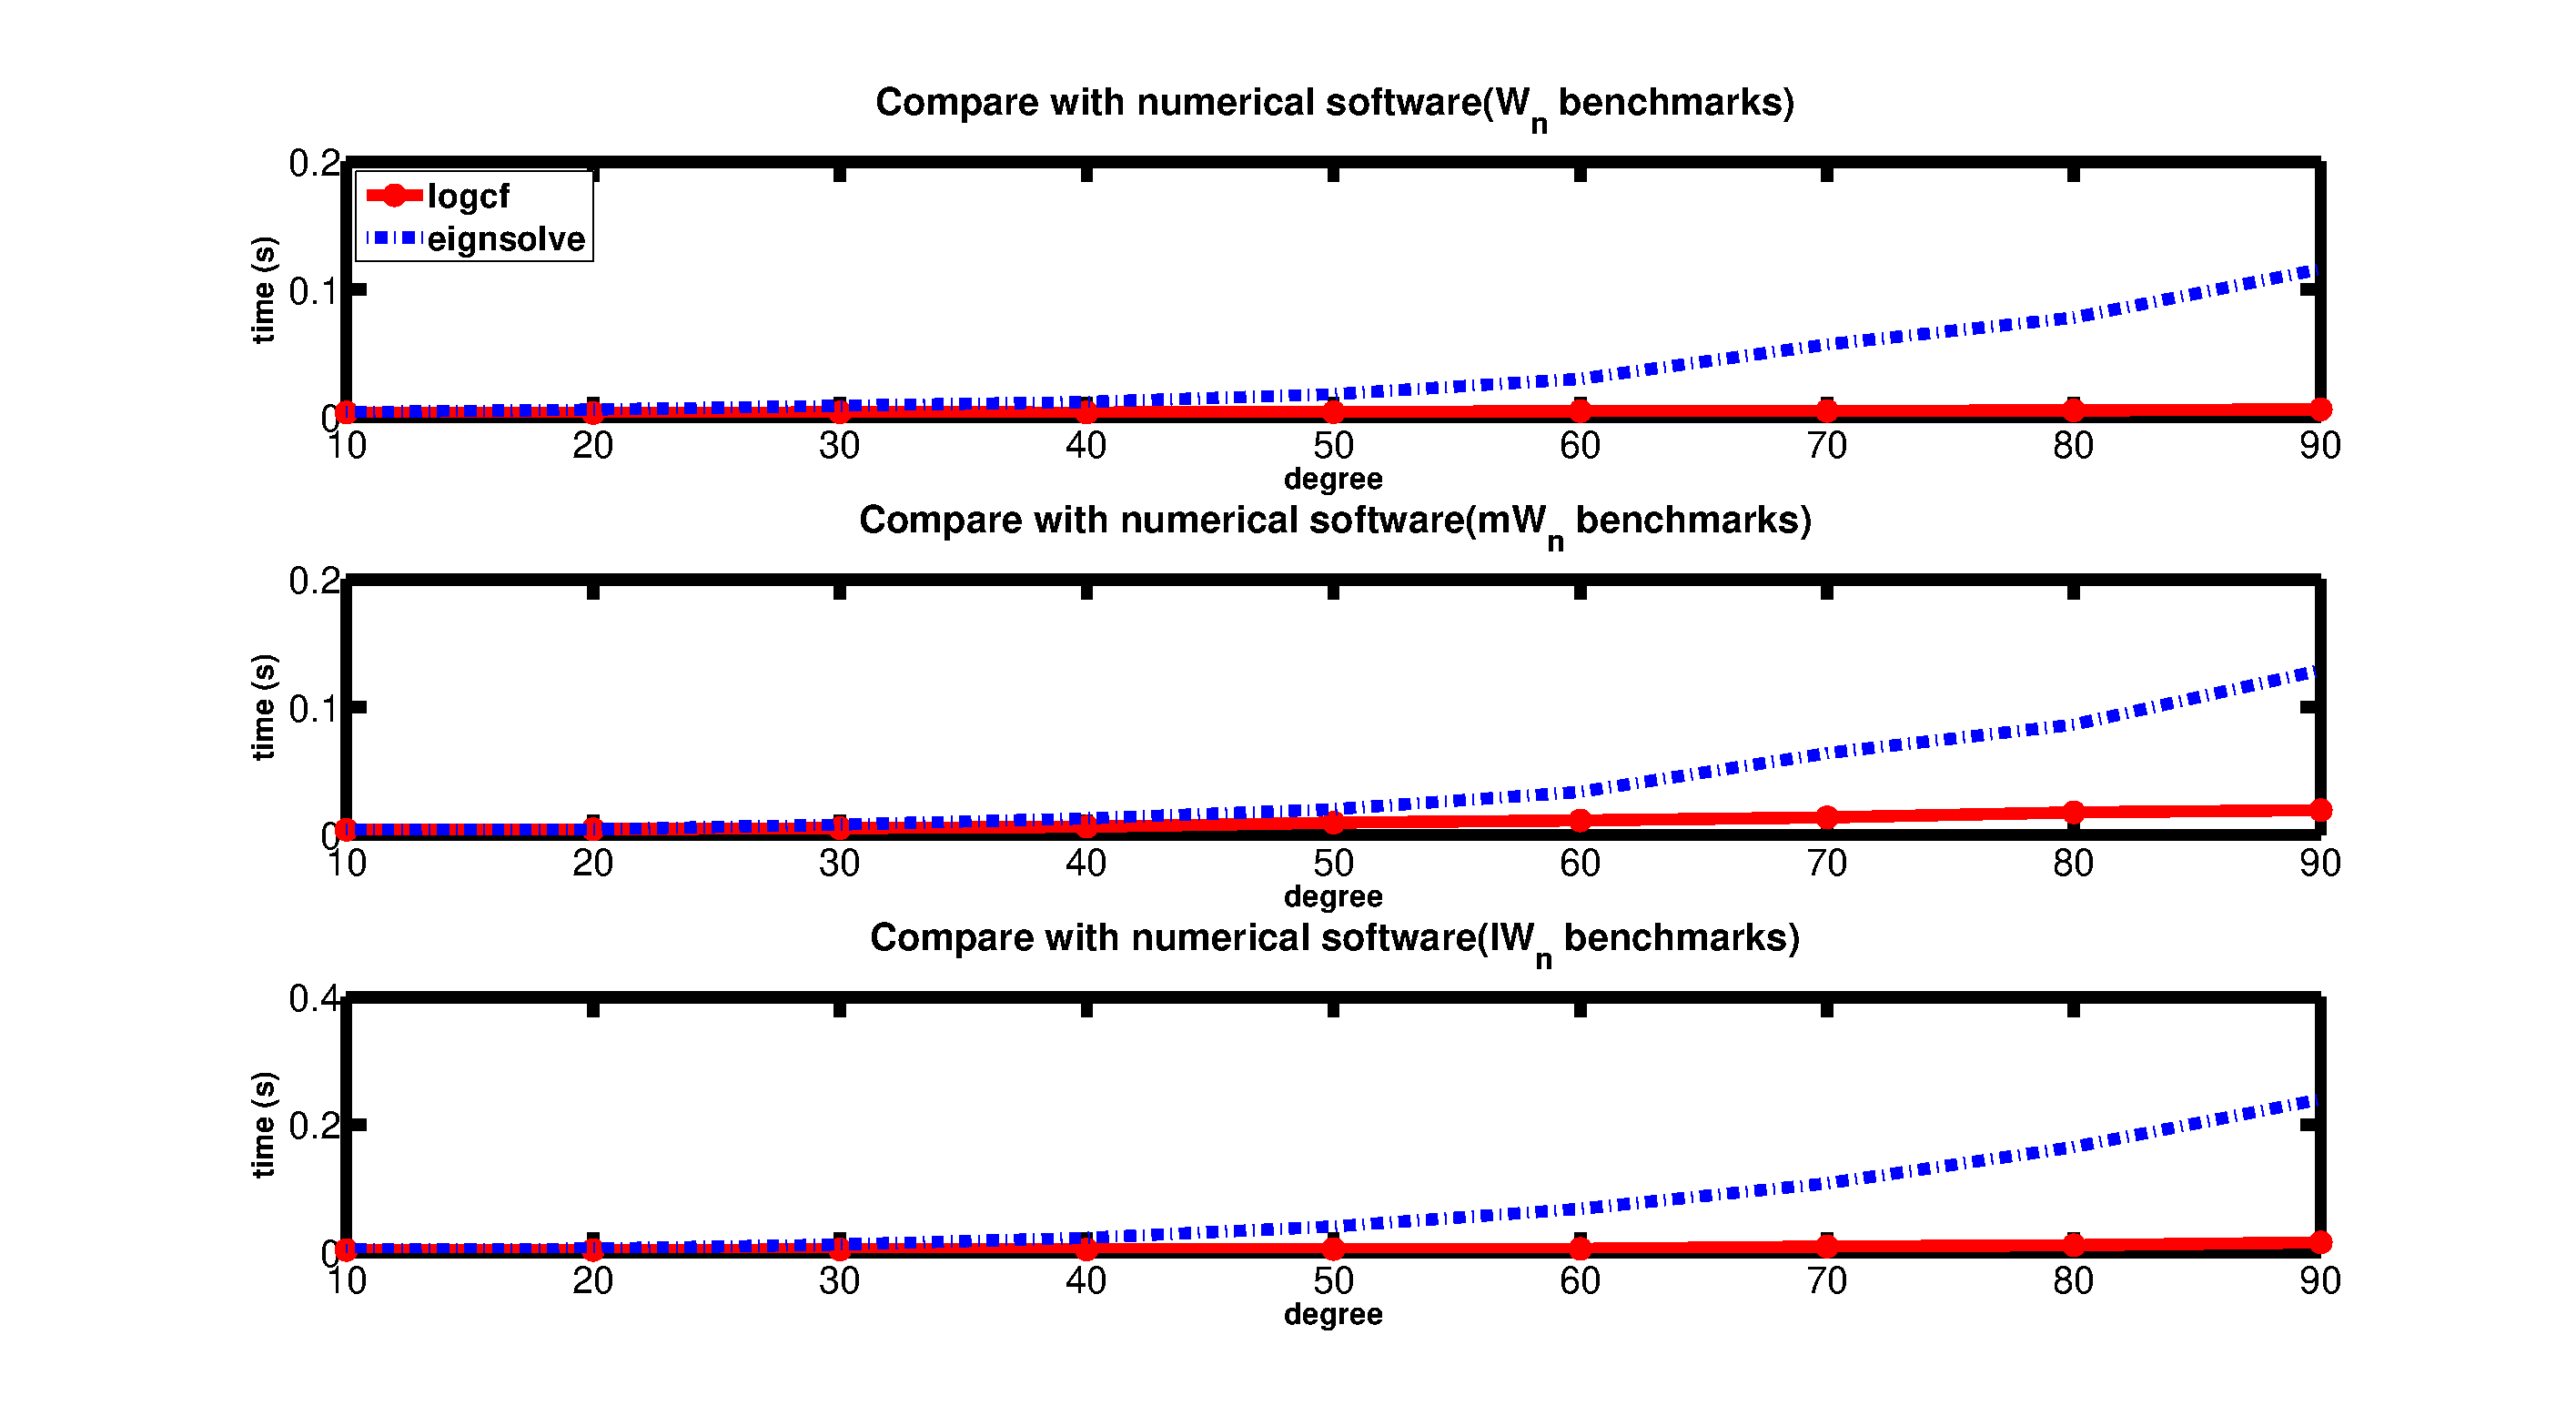
\includegraphics[width=5.4in]{com}
		\caption{ compare with numerical software  \eign\  on old environment\label{fig:1}}
	\end{centering}
\end{figure}




\begin{figure}
	\begin{centering}
		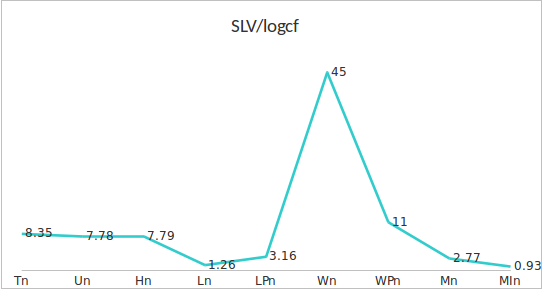
\includegraphics[width=4.4in,height=1.2in]{logcfslv}
		\caption{ Mean running time with differ kinds of polynomials under old environment\label{fig:3}}
	\end{centering}
\end{figure}





%\begin{figure}[!ht]
%	\begin{centering}
%		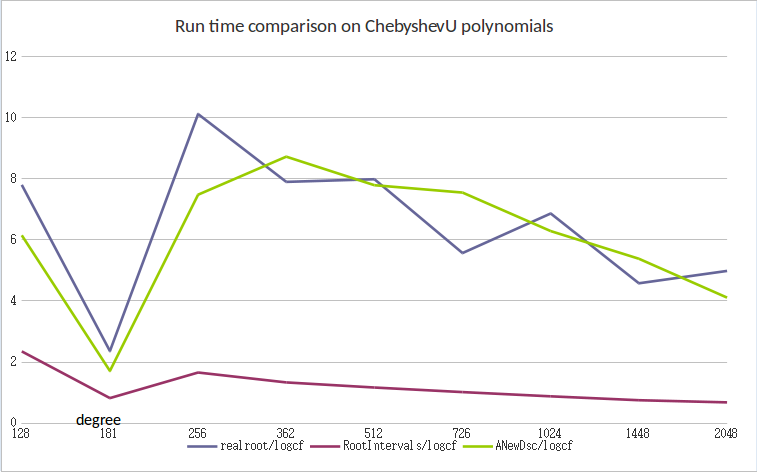
\includegraphics[width=4.4in]{Un}
%		\caption{ compare about solving ChebyshevU polynomials on new environment\label{fig:u}}
%	\end{centering}
%\end{figure}
%
%
%\begin{figure}[!ht]
%	\begin{centering}
%		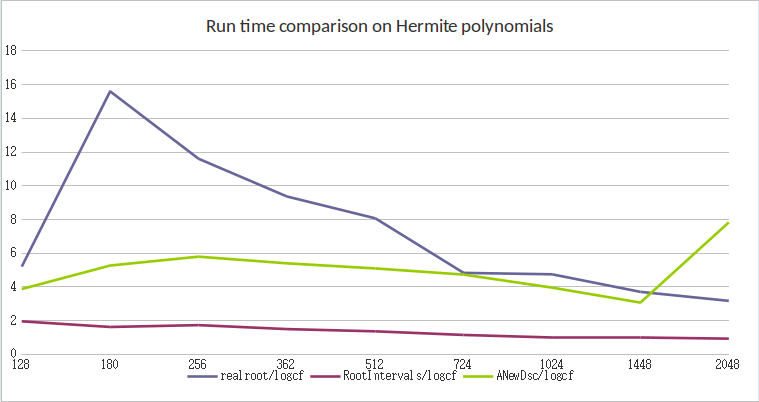
\includegraphics[width=4.4in]{Hn}
%		\caption{ compare about solving Hermite polynomials on new environment\label{fig:h}}
%	\end{centering}
%\end{figure}


%
%\begin{figure}[!ht]
%	\begin{centering}
%		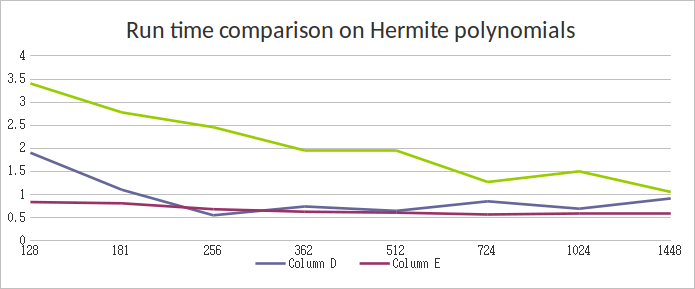
\includegraphics[width=4.4in]{Wpn}
%		\caption{ compare about solving Hermite polynomials on new environment\label{fig:h}}
%	\end{centering}
%\end{figure}


\begin{figure}
	\begin{centering}
		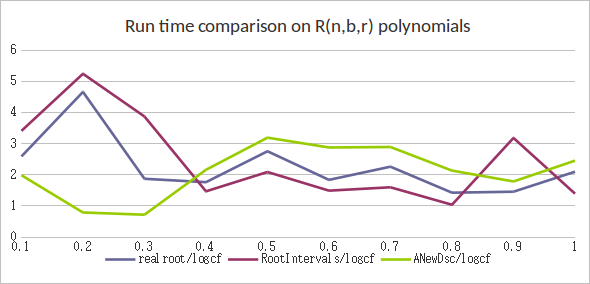
\includegraphics[width=4.4in,height=1.2in]{Rn}
		\caption{ $R(n,b,r)$ benchmarks  with differ setting on new environment\label{fig:2}}
	\end{centering}
\end{figure}



\begin{figure}
	\begin{centering}
		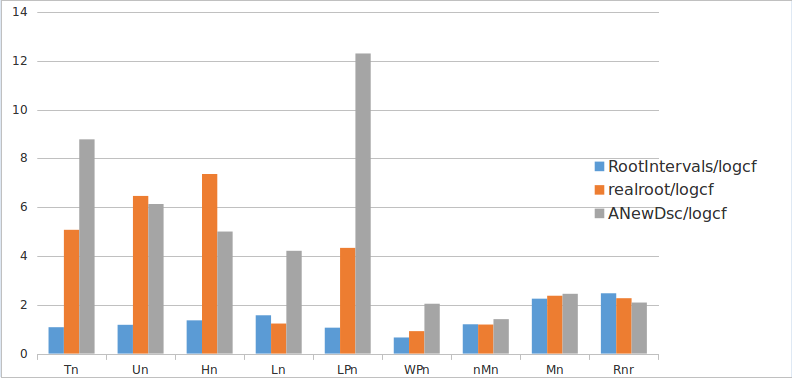
\includegraphics[width=4.4in,height=1.2in]{newresult}
		\caption{ Mean running time with differ kinds of polynomials under new environment\label{fig:newresult}}
	\end{centering}
\end{figure}

\begin{table}
	\centering
	\captionof{table}{Mean running time with differ kinds of polynomials under new environment}
	\label{tab:other}
	\begin{tabular}{|| c| c| c| c||}
		\hline
		
		\hline
		\scriptsize{Case}  &\ \  \ \ \ \ \scriptsize{$\frac{\inte }{\froot}$}\ \  \ \ \ \ \  \ \   & \ \ \ \ \  \scriptsize{$\frac{\REALROOT}{\froot}$} \ \ \ \ \  &\ \ \ \  \scriptsize{ $\frac{\AND}{\froot}$ }  \ \ \ \   \\
		\hline
		$W_n$ & 8.7 & 18.04 &  202 \\
		\hline
		$MR_n$ & 0.70 & 980 & 0.174\\
		\hline
		$MI_n$ & 0.58 & 1.89&  0.0029  \\
		\hline
		
		\hline
	\end{tabular}%}
\end{table}




\begin{table}
	\centering
	\captionof{table}{Run time(s) on $MR_n$ polynomails under new environment}
	\label{tab:and}
	\begin{tabular}{|| c| c| c| c| c ||}
		\hline
		
		\hline
		\scriptsize{Degree}  &\ \  \ \ \ \ \scriptsize{\froot}\ \  \ \  \ \   & \scriptsize{\REALROOT} &\scriptsize{\inte}  &\ \   \ \    \scriptsize{\AND}\ \ \ \   \\
		\hline
		$128$ & 0.016 & 0.734 &  0.015 &  0.02\\
		\hline
		$181$ & 0.018 & 11.154 & 0.031 & 0.038\\
		\hline
		$256$ & 0.034 & 94.849&  0.046  & 0.063\\
		\hline
		$362$ & 0.083 & >600&  0.094 & 0.11\\
		\hline
		$512$ & 0.20 &  >600 & 0.219 & 0.20  \\
		
		\hline
		$724$ & 0.55 &  >600&  0.344 & 0.42 \\
		
		\hline
		$1024$ & 1.46 & >600 & error & 0.79 \\
		
		\hline
		$1448$ & 6.48 &  >600&  error &  1.69 \\
		\hline
		$2096$ & 24.19 &  >600&  error & 3.16 \\	
		\hline
		
		\hline
	\end{tabular}%}
\end{table}









%% The Appendices part is started with the command \appendix;
%% appendix sections are then done as normal sections
%%\appendix
%% \section{}
%% \label{}

%% References
%%
%% Following citation commands can be used in the body text:
%% Usage of \cite is as follows:
%%   \cite{key}         ==>>  [#]
%%   \cite[chap. 2]{key} ==>> [#, chap. 2]
%%

%% References with bibTeX database:

%\bibliographystyle{elsarticle-num}
%\bibliography{<your-bib-database>}

%% Authors are advised to submit their bibtex database files. They are
%% requested to list a bibtex style file in the manuscript if they do
%% not want to use elsarticle-num.bst.

%% References without bibTeX database:
\section*{Acknowledgements}
The authors would like to thank Steven Fortune who sent us the source code of \eign\ and Elias P. Tsigaridas who helped us compile \cf.


%\begin{thebibliography}{00}

\bibliographystyle{abbrv}
\bibliography{realroot}



\end{document}

